\documentclass[letterpaper]{article}
\usepackage[utf8]{inputenc}
\usepackage[parfill]{parskip}    % Activate to begin paragraphs with an empty line rather than an indent
\usepackage{graphicx}
\usepackage{amssymb}
\usepackage{amsmath}
\usepackage{amsthm}
\usepackage{mathtools}
\usepackage{mathrsfs}

\usepackage{afterpage}

\usepackage{algorithm}
\usepackage{algpseudocode}

\usepackage{verse}

\newtheorem{theorem}{Theorem}[section]
\newtheorem{corollary}{Corollary}[theorem]
\newtheorem{lemma}[theorem]{Lemma}

\theoremstyle{remark}
\newtheorem*{remark}{Remark}

\usepackage{epstopdf}
\usepackage{circuitikz}
\usepackage[separate-uncertainty = true,multi-part-units=single]{siunitx}
\usepackage{booktabs}
\usepackage{enumitem}
\usepackage[toc,page]{appendix}
\usepackage{color}
\usepackage{pgfplots}
\usepackage{pgfplotstable}
\usepackage{caption}
\usepackage{subcaption}
\usepackage{url}
\usepackage{multirow}
\usepackage{makecell}
\usepackage[round]{natbib}   % omit 'round' option if you prefer square brackets
\usepackage{titling}
\usepackage{siunitx}
\usepackage{physics}

\usepackage{setspace}
% \doublespacing
\usepackage{float}


\pgfplotsset{compat=1.14}

%  Special math symbols
%       floor, ceiling, angled brackets
%-----------------------------------------------------------------------
\newcommand{\floor}[1]{\left\lfloor #1\right\rfloor}
\newcommand{\ceil}[1]{\left\lceil #1\right\rceil}
\newcommand{\etal}{\textit{et al.}}
\newcommand{\RE}{\mathbb{R}}        % real space
\newcommand{\ZZ}{\mathbb{Z}}        % integers
\newcommand{\NN}{\mathbb{N}}        % natural numbers
\newcommand{\eps}{{\varepsilon}}    % prettier epsilon
%-----------------------------------------------------------------------
%  Tighter lists
%-----------------------------------------------------------------------
\newenvironment{itemize*}% Tighter itemized list
  {\begin{itemize}%
    \setlength{\itemsep}{-0.5ex}%
    \setlength{\parsep}{0pt}}%
  {\end{itemize}}
\newenvironment{description*}% Tighter description list
  {\begin{description}%
    \setlength{\itemsep}{-0.5ex}%
    \setlength{\parsep}{0pt}}%
  {\end{description}}
\newenvironment{enumerate*}% Tighter enumerated list
  {\begin{enumerate}%
    \setlength{\itemsep}{-0.5ex}%
    \setlength{\parsep}{0pt}}%
  {\end{enumerate}}
%-----------------------------------------------------------------------
% Typing shortcuts
%-----------------------------------------------------------------------
\newcommand{\X}{\mathbb{X}}
\newcommand{\SG}{\mathbf{S}}
\newcommand{\GE}{\mathcal{G}}
\newcommand{\ST}{\,:\,}
\renewcommand{\tilde}[1]{\widetilde{#1}}
\newcommand{\diam}{\mathrm{diam}}
\newcommand{\sq}{\square}
\newcommand{\half}[1]{\frac{#1}{2}}
\newcommand{\inv}[1]{\frac{1}{#1}}
\newcommand{\alg}{\textsf{SplitReduce}}
\newcommand{\sz}[1]{\sigma_{#1}}
\newcommand{\LL}{\mathcal{L}}
\newcommand{\softOmega}{\widetilde{\Omega}} 
\newcommand{\softO}{\widetilde{O}}
\newcommand{\OO}{O^*}  %or \widetilde{O}?

\newcommand{\Null}[1]{\text{Null}(#1)}


\newcommand{\dx}{\mathrm{d}x}
\newcommand{\dy}{\mathrm{d}y}
\newcommand{\dz}{\mathrm{d}z}
\newcommand{\dt}{\mathrm{d}t}
\newcommand{\du}{\mathrm{d}u}
\newcommand{\dtheta}{\mathrm{d}\theta}
\newcommand{\dq}{\mathrm{d}q}
\newcommand{\diff}{\mathrm{d}}
\newcommand{\dV}{\mathrm{d}V}
\newcommand{\dL}{\mathrm{d}L}
\newcommand{\dA}{\mathrm{d}A}
\newcommand{\dH}{\mathrm{d}H}
\newcommand{\df}{\mathrm{d}f}
\newcommand{\dg}{\mathrm{d}g}
\newcommand{\dr}{\mathrm{d}r}
\newcommand{\dw}{\mathrm{d}w}
\newcommand{\dI}{\mathrm{d}I}

\newcommand*\len[1]{\overline{#1}}


\newcommand\note[1]{\marginpar{\textcolor{red}{#1}}}
\newcommand*{\tageq}{\refstepcounter{equation}\tag{\theequation}}

\newcommand*{\equals}{=}

\usepackage{fancyhdr}

\pgfplotscreateplotcyclelist{grayscale}{
    thick,white!10!black,mark=x,mark options=solid, dashed\\%
    thick,white!20!black,mark=o,mark options=solid\\%
}

\newcommand{\mat}[1]{\ensuremath{\begin{bmatrix}#1\end{bmatrix}}}
\newcommand{\cat}[1]{\ensuremath{\begin{vmatrix}#1\end{vmatrix}}}
\newcommand{\eqn}[1]{\begin{alignat*}{2}#1\end{alignat*}}
\newcommand{\p}[2]{\frac{\partial #1}{\partial #2}}
\newcommand*{\thus}{&\implies\quad&}

\newcommand{\answer}[1]{\framebox{$\displaystyle #1 $}}

\newcommand{\shrug}[1][]{%
\begin{tikzpicture}[baseline,x=0.8\ht\strutbox,y=0.8\ht\strutbox,line width=0.125ex,#1]
\def\arm{(-2.5,0.95) to (-2,0.95) (-1.9,1) to (-1.5,0) (-1.35,0) to (-0.8,0)};
\draw \arm;
\draw[xscale=-1] \arm;
\def\headpart{(0.6,0) arc[start angle=-40, end angle=40,x radius=0.6,y radius=0.8]};
\draw \headpart;
\draw[xscale=-1] \headpart;
\def\eye{(-0.075,0.15) .. controls (0.02,0) .. (0.075,-0.15)};
\draw[shift={(-0.3,0.8)}] \eye;
\draw[shift={(0,0.85)}] \eye;
% draw mouth
\draw (-0.1,0.2) to [out=15,in=-100] (0.4,0.95); 
\end{tikzpicture}}


\pagestyle{fancy}
\fancyhf{}
\rhead{Rahul Arya}
\lhead{EE 16B}
\cfoot{\thepage}

\title{Lecture 23 - Notes}
\author{Rahul Arya}
\date{April 2019}
\begin{document}

\maketitle

\section{Overview}
Over the next few lectures, we will begin to study discrete signals in the frequency domain. Of course, signals in the frequency domain are by their construction defined over continuous time. Thus, we need some way to convert a discrete-time signal into a continuous-time one, that preserves its important properties. We will address this problem, known as \emph{interpolation}, in this lecture.

\section{Properties of an Interpolation}
In the above definition of interpolation, there are two main ambiguities: what exactly is meant by a ``discrete-time signal'', and what are its important properties that should be preserved after interpolation? 

We define a discrete-time signal to be a series of measurements (known as \emph{samples}) of some underlying continuous-time signal, as illustrated below:
\begin{center}
\begin{tikzpicture}
\begin{axis}[
    xlabel=$t$, ylabel=$ $,
    xmin=-0.5, xmax=4.5,
    ymin=0, ymax=12,
    legend style={at={(1.02,1)},anchor=north west},
 ]
\addplot [domain=-1:5, color=blue, samples=500, dashed] {4*x^2 - x^3 + 1};
\addlegendentry{Continuous-time signal};
\addplot +[domain=0:5, color=red, ycomb] plot coordinates {(0, 1) (1, 4) (2, 9) (3, 10) (4, 1)};
\addlegendentry{Discrete-time samples};
% \addplot [domain=10^(-2):1] {x};
% \addplot [domain=1:10^(2)] {1 / x};
% \addlegendentry{Approximation};
\end{axis}
\end{tikzpicture}
\end{center}
In almost all cases (including all the cases we will consider here), our samples will be made at a constant interval $\Delta$. For instance, in the above figure, $\Delta = 1$. 

Interpolation can be thought of as the task of (approximately) recovering the original continuous-time signal from our discrete samples. An immediate consequence of this is that an interpolated signal should pass through all of its sample points, since we know that the original signal certainly did. In fact, we will consider this property to be the only requirement that an interpolation must satisfy for now, though we will introduce more requirements in the future. Thus, we can view interpolation simply to be the construction of a continuous-time function that passes through all our sample points.

\section{Simple Interpolations}
The problem of interpolation doesn't sound too hard - intuitively, it is trivial to construct a continuous-time function passing through a given set of points - just join them together with straight lines! This interpolation is known as \emph{piecewise linear} interpolation, and is a very natural construction. For instance, in the above figure, we obtain the piecewise-linear interpolation
\begin{center}
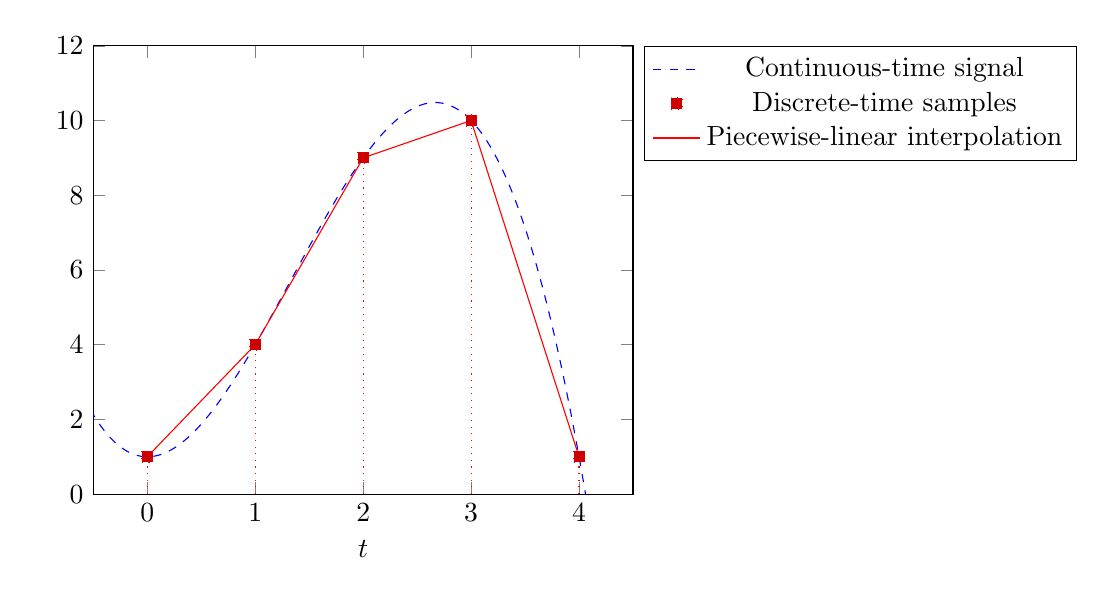
\begin{tikzpicture}
\begin{axis}[
    xlabel=$t$, ylabel=$ $,
    xmin=-0.5, xmax=4.5,
    ymin=0, ymax=12,
    legend style={at={(1.02,1)},anchor=north west},
 ]
\addplot [domain=-1:5, color=blue, samples=500, dashed] {4*x^2 - x^3 + 1};
\addlegendentry{Continuous-time signal};
\addplot +[domain=0:5, color=red, ycomb, dotted] plot coordinates {(0, 1) (1, 4) (2, 9) (3, 10) (4, 1)};
\addlegendentry{Discrete-time samples};
\addplot [domain=0:5, color=red] coordinates {(0, 1) (1, 4) (2, 9) (3, 10) (4, 1)};
\addlegendentry{Piecewise-linear interpolation};
% \addplot [domain=10^(-2):1] {x};
% \addplot [domain=1:10^(2)] {1 / x};
% \addlegendentry{Approximation};
\end{axis}
\end{tikzpicture}
\end{center}
Our piecewise-linear interpolation seems to work fairly well at approximating the original signal, as we intuitively expected, but is less accurate near intervals where the continuous-time signal changes slope rapidly, such as near the local maximum in the above figure.

Another, even simpler, interpolation would be to just forget about trying to ``interpolate'' at all, and just retain the value of the previous sample point. This technique, known as \emph{zero-order hold} interpolation, produces the following result:
\begin{center}
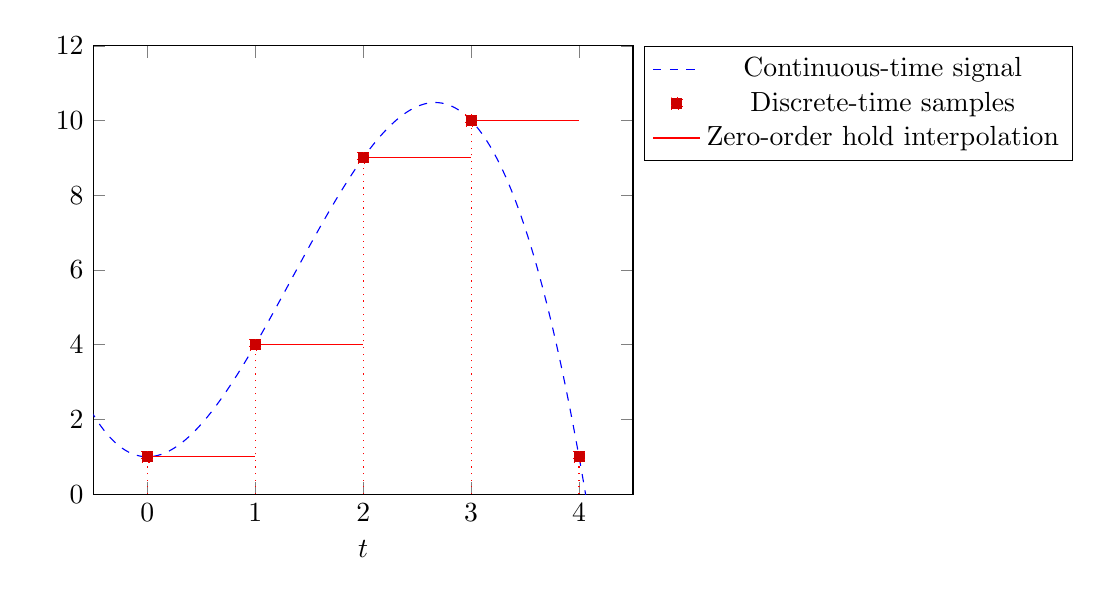
\begin{tikzpicture}
\begin{axis}[
    xlabel=$t$, ylabel=$ $,
    xmin=-0.5, xmax=4.5,
    ymin=0, ymax=12,
    legend style={at={(1.02,1)},anchor=north west},
 ]
\addplot [domain=-1:5, color=blue, samples=500, dashed] {4*x^2 - x^3 + 1};
\addlegendentry{Continuous-time signal};
\addplot +[domain=0:5, color=red, ycomb, dotted] plot coordinates {(0, 1) (1, 4) (2, 9) (3, 10) (4, 1)};
\addlegendentry{Discrete-time samples};
\addplot [domain=0:5, color=red] coordinates {(0, 1) (1, 1)};
\addplot [domain=0:5, color=red] coordinates {(1, 4) (2, 4)};
\addplot [domain=0:5, color=red] coordinates {(2, 9) (3, 9)};
\addplot [domain=0:5, color=red] coordinates {(3, 10) (4, 10)};
\addlegendentry{Zero-order hold interpolation};
% \addplot [domain=10^(-2):1] {x};
% \addplot [domain=1:10^(2)] {1 / x};
% \addlegendentry{Approximation};
\end{axis}
\end{tikzpicture}
\end{center}
Notice that this approximation is quite a bit worse than our piecewise-linear interpolation, but still passes through all our sample points and at least somewhat retains the shape of the original signal.

\section{Basis Functions}
As it turns out, the previous two interpolations can both be described as examples of a broader class of interpolations, which are based on the idea of \emph{basis functions}. Basis function interpolations have the following two additional properties, which are both fairly natural:
\begin{itemize}
    \item The interpolation produced from a linear combination of two discrete-time signals is the same linear combination of the interpolation of the two discrete-time samples. In other words, interpolation can be thought of as a linear transformation of their input discrete-time signals onto the space of continuous functions.
    \item Interpolations do not depend on a reference time. That is to say, if we shift a discrete-time signal forward by $k$ samples, its interpolation will shift forward by $k\Delta$ time.
\end{itemize}
Observe that the above two properties are clearly satisfied by both the piecewise-linear and zero-order hold interpolations we saw earlier.

Now, we define the \emph{basis function} of a particular interpolation to be the interpolation $\phi(t)$ of the discrete signal with sample points
\[
    \ldots, (-2\Delta, 0), (-\Delta, 0), (0, 1), (\Delta, 0), (2\Delta, 0), \ldots
\]
In other words, it is the interpolation of a discrete signal that is $0$ everywhere except at $t = 0$, where it is $1$. We claim that we can use this basis function, along with the known properties of basis function interpolations, to interpolate \emph{any} discrete-time signal. In other words, the choice of basis function $\phi(t)$ fully determines the behavior of our interpolation.

To prove the above claim, let our arbitrary input discrete-time signal be $\vec{x}$. Let $\vec{b}_i$ be a discrete-signal that is $0$ everywhere except at $t = i\Delta$, where it is $1$. By the second property of basis-function interpolations, it is clear that
\eqn{
    && \mathrm{Interpolate}(\vec{b}_0) &= \phi(t) \\
    \thus \mathrm{Interpolate}(\vec{b}_k) &= \phi(t - k\Delta).
}
It should be clear that we can choose coefficients $\alpha_i$ such that
\[
    \vec{x} = \sum_i \alpha_i \vec{b}_i,
\]
treating $\vec{x}$ to be of finite length.

Now, we can apply the first property of basis-function interpolations, to see that
\eqn{
    && \mathrm{Interpolate}(\vec{x}) &= \mathrm{Interpolate}(\sum_i \alpha_i \vec{b}_i) \\
    &&&= \sum_i \alpha_i \cdot \mathrm{Interpolate}(\vec{b}_i).
}
Combining this result and the result immediately preceding it, we therefore find that
\[
    \mathrm{Interpolate}(\vec{x}) = \sum_i \alpha_i \cdot \phi(t - i\Delta),
\]
so we have constructed the interpolation of an arbitrary discrete-time signal from just our basis function, proving our claim.

\section{Example Basis Functions}
Let's apply the above general result to the particular examples of piecewise-linear and zero-order hold interpolations, in order to gain some intuition for this new way of thinking about interpolation. Recall that both these types of interpolation satisfy the two additional requirements of basis-function interpolations, so their basis functions must exist.

Consider piecewise-linear interpolation first. By the definition of a basis function, we need to compute the piecewise-linear interpolation of $\vec{b}_0$, which we see graphically is as follows:
\begin{center}
\begin{tikzpicture}
\begin{axis}[
    xlabel=$t/\Delta$, ylabel=$ $,
    xmin=-2.5, xmax=2.5,
    ymin=-1, ymax=2,
    legend style={at={(1.02,1)},anchor=north west},
 ]
\addplot +[domain=0:5, color=red, ycomb, dotted] plot coordinates {(-2, 0) (-1, 0) (0, 1) (1, 0) (2, 0)};
\addlegendentry{$\vec{b}_0$};
\addplot [domain=0:5, color=red] coordinates {(-2, 0) (-1, 0) (0, 1) (1, 0) (2, 0)};
\addlegendentry{$\phi(t)$};
% \addplot [domain=10^(-2):1] {x};
% \addplot [domain=1:10^(2)] {1 / x};
% \addlegendentry{Approximation};
\end{axis}
\end{tikzpicture}
\end{center}
Algebraically, we see that
\[
    \phi(t) = \begin{cases}
    0, & \text{for } t < -\Delta \\
    1 + t, & \text{for } -\Delta \le t < 0 \\
    1 - t, & \text{for } 0 \le t < \Delta \\
    0, & \text{for } t \ge \Delta
  \end{cases}.
\]
Solving for the interpolation of a set of sample points with $\Delta = 1$ by evaluating the summation we obtained in the previous section, we see that it is equivalent to summing the following interpolations graphically
\begin{center}
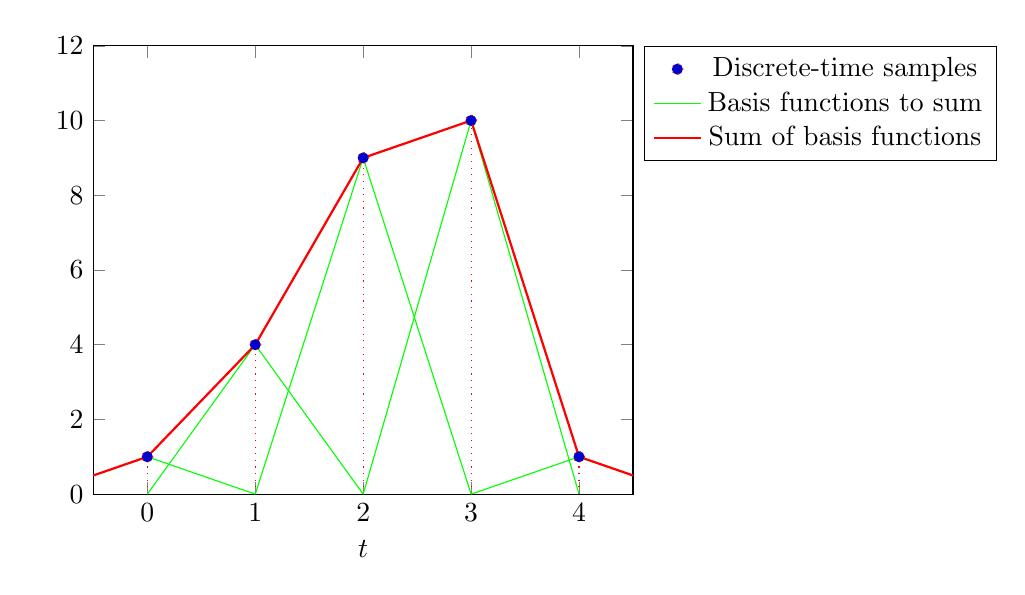
\begin{tikzpicture}
\begin{axis}[
    xlabel=$t$, ylabel=$ $,
    xmin=-0.5, xmax=4.5,
    ymin=0, ymax=12,
    legend style={at={(1.02,1)},anchor=north west},
 ]
\addplot +[domain=0:5, color=red, ycomb, dotted] plot coordinates {(0, 1) (1, 4) (2, 9) (3, 10) (4, 1)};
\addlegendentry{Discrete-time samples};
\addplot [domain=0:5, color=green,forget plot] coordinates {(-1, 0) (0, 1) (1, 0)};
\addplot [domain=0:5, color=green,forget plot] coordinates {(0, 0) (1, 4) (2, 0)};
\addplot [domain=0:5, color=green,forget plot] coordinates {(1, 0) (2, 9) (3, 0)};
\addplot [domain=0:5, color=green,forget plot] coordinates {(2, 0) (3, 10) (4, 0)};
\addplot [domain=0:5, color=green] coordinates {(3, 0) (4, 1) (5, 0)};
\addlegendentry{Basis functions to sum};
\addplot [domain=0:5, color=red, thick] coordinates {(-1, 0) (0, 1) (1, 4) (2, 9) (3, 10) (4, 1) (5, 0)};
\addlegendentry{Sum of basis functions};
% \addplot [domain=10^(-2):1] {x};
% \addplot [domain=1:10^(2)] {1 / x};
% \addlegendentry{Approximation};
\end{axis}
\end{tikzpicture}
\end{center}
Notice that the sum of the scaled and translated basis functions yields exactly the piecewise-linear interpolation that we saw earlier, demonstrating how piecewise-linear interpolation can be thought of as summing basis functions.

Now, let's look at zero-order hold interpolation in a similar manner. Computing the zero-order hold interpolation of $\vec{b}_0$, we graphically obtain:
\begin{center}
\begin{tikzpicture}
\begin{axis}[
    xlabel=$t/\Delta$, ylabel=$ $,
    xmin=-2.5, xmax=2.5,
    ymin=-1, ymax=2,
    legend style={at={(1.02,1)},anchor=north west},
 ]
\addplot +[domain=0:5, color=red, ycomb, dotted] plot coordinates {(-2, 0) (-1, 0) (0, 1) (1, 0) (2, 0)};
\addlegendentry{$\vec{b}_0$};
\addplot [domain=0:5, color=red] coordinates {(-2, 0) (-1, 0) (0, 0)};
\addplot [domain=0:5, color=red] coordinates {(0, 1) (1, 1)};
\addplot [domain=0:5, color=red] coordinates {(1, 0) (2, 0)};
\addlegendentry{$\phi(t)$};
% \addplot [domain=10^(-2):1] {x};
% \addplot [domain=1:10^(2)] {1 / x};
% \addlegendentry{Approximation};
\end{axis}
\end{tikzpicture}
\end{center}
Algebraically, we see that
\[
    \phi(t) = \begin{cases}
    0, & \text{for } t < 0 \\
    1, & \text{for } 0 \le t < \Delta \\
    0, & \text{for } t \ge \Delta
  \end{cases}.
\]
And evaluating the summation from the previous section in order to compute the zero-order hold interpolation of an arbitrary discrete-time signal with $\Delta = 1$, we see that it is equivalent to summing the following interpolations graphically:
\begin{center}
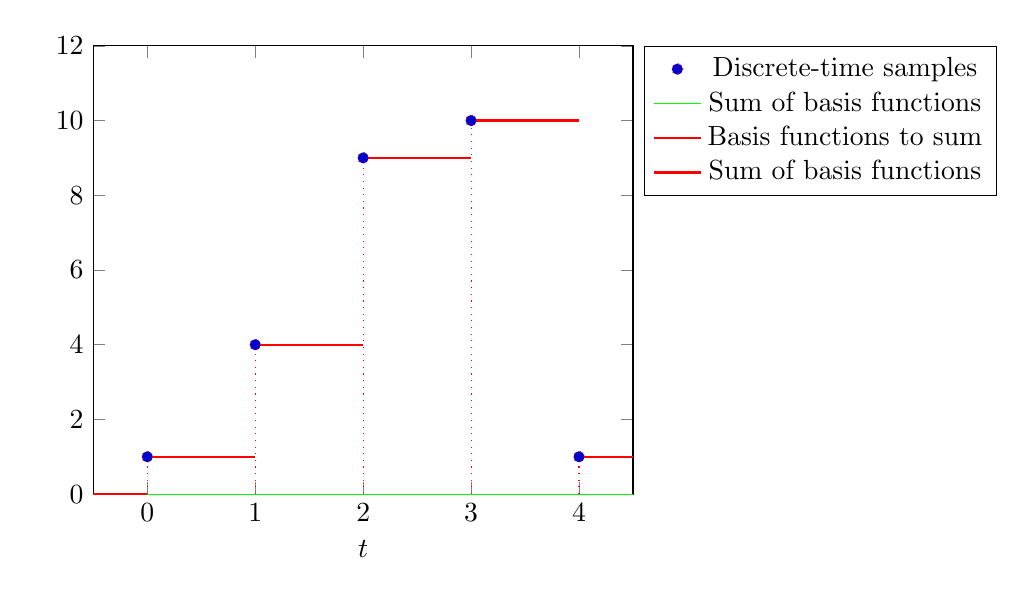
\begin{tikzpicture}
\begin{axis}[
    xlabel=$t$, ylabel=$ $,
    xmin=-0.5, xmax=4.5,
    ymin=0, ymax=12,
    legend style={at={(1.02,1)},anchor=north west},
 ]
\addplot +[domain=0:5, color=red, ycomb, dotted] plot coordinates {(0, 1) (1, 4) (2, 9) (3, 10) (4, 1)};
\addlegendentry{Discrete-time samples};
\addplot [domain=0:5, color=green] coordinates {(-1, 0) (6, 0)};
\addlegendentry{Sum of basis functions};
\addlegendentry{Basis functions to sum};
\addplot [domain=0:5, color=red, thick] coordinates {(-1, 0) (0, 0)};
\addplot [domain=0:5, color=red, thick] coordinates {(0, 1) (1, 1)};
\addplot [domain=0:5, color=red, thick] coordinates {(1, 4) (2, 4)};
\addplot [domain=0:5, color=red, thick] coordinates {(2, 9) (3, 9)};
\addplot [domain=0:5, color=red, thick] coordinates {(3, 10) (4, 10)};
\addplot [domain=0:5, color=red, thick] coordinates {(4, 1) (5, 1)};
\addlegendentry{Sum of basis functions};
% \addplot [domain=10^(-2):1] {x};
% \addplot [domain=1:10^(2)] {1 / x};
% \addlegendentry{Approximation};
\end{axis}
\end{tikzpicture}
\end{center}
Again, we obtain exactly the same interpolation as before, when we calculated the zero-order hold interpolation directly.

\section{Sinc Interpolation}
The motivation behind the general idea of basis-function interpolation is that we can now construct new interpolations easily, by picking an appropriate basis function. Recall that a basis function $\phi(t)$ was defined to be the interpolation of $\vec{b}_0$. Thus, by the first property of interpolations that we established at the beginning,
\[
    \phi(0) = 1 \text{ and } (\forall k \ne 0) \phi(\Delta k) = 0,
\]
since an interpolation must pass through all the provided sample points. But no further restrictions are present, meaning that \emph{any} function satisfying this condition can give rise to a new basis-function interpolation.

Furthermore, notice (though we will not prove it explicitly) that an interpolation will be non-differentiable when its basis function is itself non-differentiable. For instance, observe that the basis function for piecewise-linear interpolation had three non-differentiable points (at $t = -1$, $t = 0$, and $t = 1$), so it produces interpolations that are themselves non-differentiable at some points. 

Similarly, an interpolation will be discontinuous only if its basis function is itself discontinuous. Since the piecewise-linear basis function was continuous, the piecewise-linear interpolations of arbitrary discrete-time signals were all continuous as well. However, since the zero-order hold basis function was discontinuous at $t = 0$ and $t = 1$, it gave rise to discontinuous interpolations as well.

More generally, most properties that are preserved under linear transformations (such as differentiability, continuity, boundedness, or continuity) are true of a basis-function interpolation exactly when they are true of the basis function itself. It is often the case that we want a method of producing a smooth interpolation from a discrete-signal - for instance, smoothness turns out to be useful when performing frequency analysis. 

But to produce one, we need to have a smooth basis function - since neither of the two functions we currently have are differentiable, they are clearly not suitable candidates. Instead, we will propose the \emph{sinc} basis function, defined as
\[
    \phi(t) = \frac{\sin{(\pi t / \Delta)}}{\pi t / \Delta}
\]
for all $t \ne 0$, with the discontinuity at $t = 0$ removed by defining $\phi(0) = 1$\footnote{It is straightforward to see that this value will indeed remove the discontinuity.}. Observe that for any integer $k \ne 0$,
\[
    \phi(\Delta k) = \frac{\sin{(\pi (k\Delta) / \Delta)}}{\pi (k\Delta) / \Delta} = \frac{\sin(k\pi)}{k\pi} = 0,
\]
so $\phi(t)$ satisfies the requirements of a basis function. Plotting this function with $\Delta = 1$, we obtain
\begin{center}
\begin{tikzpicture}
\begin{axis}[
    xlabel=$t$, ylabel=$ $,
    xmin=-3, xmax=3,
    ymin=-0.5, ymax=1.5,
    legend style={at={(1.02,1)},anchor=north west},
 ]
\addplot +[domain=0:5, color=red, ycomb, dotted] plot coordinates {(-2, 0) (-1, 0) (0, 1) (1, 0) (2, 0)};
\addlegendentry{$\vec{b}_0$};
\addplot [domain=-3:3, samples=500, color=red] {sin(180 * x ) / (pi * x)};
\addlegendentry{$\phi(t)$};
% \addplot [domain=10^(-2):1] {x};
% \addplot [domain=1:10^(2)] {1 / x};
% \addlegendentry{Approximation};
\end{axis}
\end{tikzpicture}
\end{center}
Although we will not prove it explicitly, it is not hard to show that $\phi(t)$ is also smooth, as we had hoped.

Now, we can try using this basis function to construct interpolations. Our aim will be to produce interpolations that smoothly move between our sample points. For an arbitrary set of sample points with $\Delta = 1$, we obtain
\begin{center}
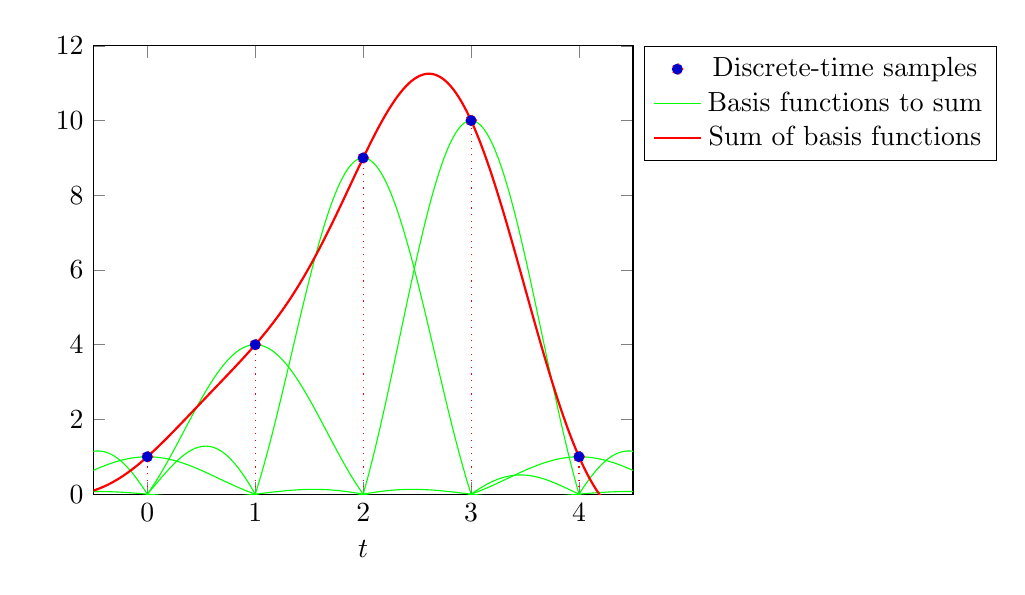
\begin{tikzpicture}
\begin{axis}[
    xlabel=$t$, ylabel=$ $,
    xmin=-0.5, xmax=4.5,
    ymin=0, ymax=12,
    legend style={at={(1.02,1)},anchor=north west},
 ]
\addplot +[domain=0:5, color=red, ycomb, dotted] plot coordinates {(0, 1) (1, 4) (2, 9) (3, 10) (4, 1)};
\addlegendentry{Discrete-time samples};
\addplot [domain=-1:5, color=green, forget plot, samples=500] {1 * sin(180 * (x - 0)) / (pi * (x - 0))};
\addplot [domain=-1:5, color=green, forget plot, samples=500] {4 * sin(180 * (x - 1)) / (pi * (x - 1))};
\addplot [domain=-1:5, color=green, forget plot, samples=500] {9 * sin(180 * (x - 2)) / (pi * (x - 2))};
\addplot [domain=-1:5, color=green, forget plot, samples=500] {10 * sin(180 * (x - 3)) / (pi * (x - 3))};
\addplot [domain=-1:5, color=green, samples=500] {sin(180 * (x - 4)) / (pi * (x - 4))};
\addlegendentry{Basis functions to sum};
\addplot [domain=-1:5, color=red, thick, samples=500] {1 * sin(180 * (x - 0)) / (pi * (x - 0)) + 4 * sin(180 * (x - 1)) / (pi * (x - 1)) + 9 * sin(180 * (x - 2)) / (pi * (x - 2)) + 10 * sin(180 * (x - 3)) / (pi * (x - 3)) + sin(180 * (x - 4)) / (pi * (x - 4))};
\addlegendentry{Sum of basis functions};
% \addplot [domain=10^(-2):1] {x};
% \addplot [domain=1:10^(2)] {1 / x};
% \addlegendentry{Approximation};
\end{axis}
\end{tikzpicture}
\end{center}
Observe that the interpolation passes through all the sample points (as we showed it must) much more naturally than did either of our previous two interpolations. 

\section{Polynomial Interpolation}
Recall from EE16A that we could construct a polynomial of minimum degree that passed through a given set of points, if one existed. It is a natural question to ask whether this method can be adapted into another way of constructing a smooth interpolation of a discrete-time signal (since all polynomials are clearly smooth). Imagine that we had $n$ sample points, from $t = 0$ to $t = (n-1)\Delta$, and wished to construct a polynomial of degree $d$ passing through all these $n$ sample points. Let such a polynomial be
\[
    p(t) = a_0 + a_1t + a_2t^2 + \ldots + a_dt^d,
\]
and let our sample points be
\[
    (0, y_0), (\Delta, y_1), \ldots, ((n-1)\Delta, y_{n-1}).
\]
For convenience, let $x_i = \Delta i$ for integer $0 \le i < n$. Since $p(x_i) = y_i$ for all our sample points, we obtain the system of linear equations
\eqn{
    && a_0 + a_1x_0 + a_2x_0^2 + \ldots + a_dx_0^d &= y_0 \\
    && a_0 + a_1x_1 + a_2x_1^2 + \ldots + a_dx_1^d &= y_1 \\
    &&& \vdots \\
    && a_0 + a_1x_{n-1} + a_2x_{n-1}^2 + \ldots + a_dx_{n-1}^d &= y_{n-1},
}
which can be rewritten in matrix form as
\[
    \mat{
        1 & x_0 & x_0^2 & \ldots & x_0^d \\
        1 & x_1 & x_1^2 & \ldots & x_1^d \\ 
        \vdots & \vdots & \vdots & \ddots & \vdots \\ 
        1 & x_{n-1} & x_{n-1}^2 & \ldots & x_{n-1}^d
    } \mat{a_0 \\ a_1 \\ \vdots \\ a_d} = \mat{y_0 \\ y_1 \\ \vdots \\ y_{n-1}}.
\]
Clearly, for a unique solution to always exist, the matrix on the left-hand-side must be square, so $n = d + 1$. In that case, that matrix is known as a \emph{Vandermonde matrix}. An important property of Vandermonde matrices is that, assuming all the $x_i$ are distinct, they will always be invertible, so we can always solve for the $a_i$, as we expected.

The question remains - what does such a polynomial look like, and how does it compare to our earlier methods of interpolation (specifically, sinc interpolation). Unfortunately, while polynomial interpolation can work in some cases, it turns out that in general it performs poorly, particularly near the edges of the samples, where the interpolated polynomial starts to rise and fall rapidly to pass through all the sample points. This behavior is known as \emph{Runge's phenomenon}, though we will not study it in great detail for this course.

Nonetheless, we can see an example of this in the following polynomial interpolation of a discrete-time signal with $\Delta = 0.2$:
\begin{center}
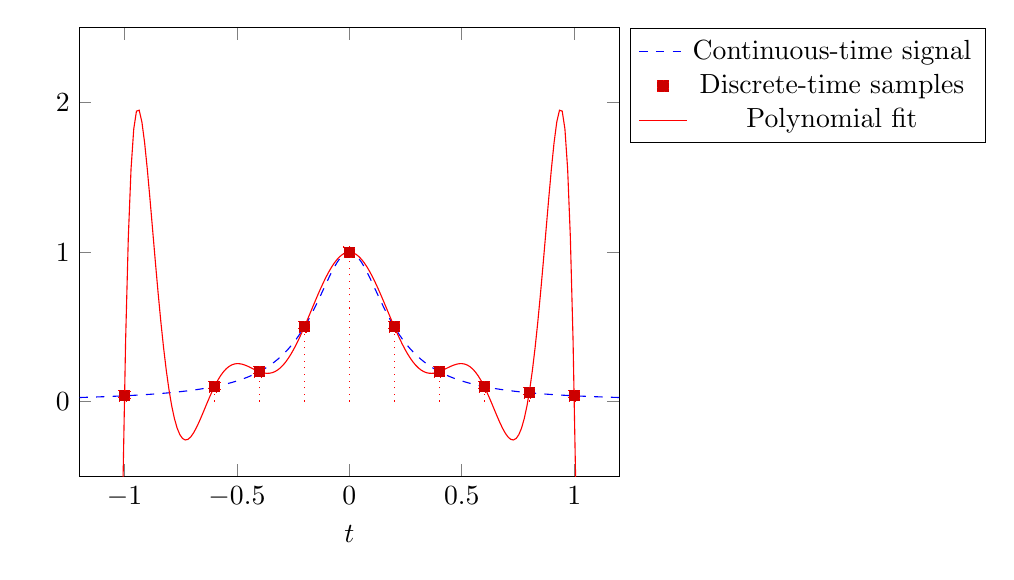
\begin{tikzpicture}
\begin{axis}[
    xlabel=$t$, ylabel=$ $,
    xmin=-1.2, xmax=1.2,
    ymin=-0.5, ymax=2.5,
    legend style={at={(1.02,1)},anchor=north west},
 ]
\addplot [domain=-1.2:1.2, color=blue, samples=200, dashed] {1/(1 + 25 * x * x)};
\addlegendentry{Continuous-time signal};
\addplot +[domain=0:5, color=red, ycomb, dotted] plot coordinates {
                                                                (-1, 1/(1 + 25 * 1^2) 
                                                                (-0.6, 1/(1 + 25 * 0.6^2) 
                                                                (-0.4, 1/(1 + 25 * 0.4^2) 
                                                                (-0.2, 1/(1 + 25 * 0.2^2) 
                                                                (0, 1/(1 + 25 * 0^2) 
                                                                (0.2, 1/(1 + 25 * 0.2^2) 
                                                                (0.4, 1/(1 + 25 * 0.4^2)
                                                                (0.6, 1/(1 + 25 * 0.6^2) 
                                                                (0.8, 1/(1 + 25 * 0.8^2) 
                                                                (1, 1/(1 + 25 * 1)};
\addlegendentry{Discrete-time samples};
\addplot [domain=-1.2:1.2, color=red, samples=200] {2.6362062029803235e-11 *x^ 11 +-220.94174208145742 *x^ 10 +-5.552193884451033e-11 *x^ 9 +494.90950226246065 *x^ 8 +3.938177994589497e-11 *x^ 7 +-381.43382352942115 *x^ 6 +-1.1432207904482855e-11 *x^ 5 +123.35972850678912 *x^ 4 +1.2449895989454678e-12 *x^ 3 +-16.85520361990966 *x^ 2 +3.227721070222798e-14 *x^ 1 +0.9999999999999528 *x^ 0};
\addlegendentry{Polynomial fit};
% \addplot [domain=10^(-2):1] {x};
% \addplot [domain=1:10^(2)] {1 / x};
% \addlegendentry{Approximation};
\end{axis}
\end{tikzpicture}
\end{center}
The polynomial fit, though it passes through the points, is extremely poor near the edges, oscillating violently. As a consequence, we will typically use sinc interpolation when we require a smooth interpolation, unless there is a good reason to do otherwise.

\end{document}
